\chapter{PySPH: Design Philosophy}

PySPH ~\cite{prabhu_puri} ~ is ~ an ~ open-source, ~ objected ~ oriented ~ Python\\ \cite{python} based framework for SPH simulations with the performance critical portions implemented in Cython \cite{cython}. The PySPH tool is flexible, user-friendly and allows for quick prototyping and extension to new problems. In this chapter, an broad outline of the PySPH tool is laid out\footnote[3]{further details of specifics related to new implementations will be discussed as and when encountered}.

\section{Abstractions for Numerical Implementation}

In order to motivate and explain the abstractions made for the numerical implementation, we consider a general SPH discretization (Equations \eqref{eq:Disc_SPH}) for the continuum equations for Mass, Momentum and Energy balance (Equations \eqref{eq:balance_laws}):

\begin{eqnarray} \label{eq:balance_laws}
\frac{D\rho}{Dt} &=& -\frac{1}{\rho} \nabla \cdot \vec{v} \nonumber \\
\frac{D{\vec{v}}}{Dt}&=&\vec{{\bf{k}}} + \frac{1}{\rho} \frac{\partial \tau^{lm}}{\partial x_m} \hat{l} \\
\frac{D{\it{e}}}{Dt}&=& -\frac{1}{\rho}\nabla \cdot \vec{q} + \frac{1}{\rho}\frac{\partial {\it{v}^{l}} }{\partial x_m}\tau^{lm} \nonumber
\end{eqnarray}

{\raggedright{where,}}\\
$\frac{D}{Dt}(\varphi) = $ Material Derivative of the field variable $\varphi = \left(\frac{\partial}{\partial t} + \vec{v}\cdot\nabla\right)(\varphi)$ \\
$\rho = $ Mass per unit volume in the limit that volume goes to zero at any point in the continuum\\
$\vec{v} = $ Velocity vector associated with a point particle\\
$\vec{{\bf{k}}} = $ Body Force per unit mass\\
$\tau^{lm} = $ Components of the stress tensor field\\
$e = $ Internal Energy per unit mass\\
$\vec{q} = $ Heat Flux Vector (heat energy transferred per unit time per unit area along the direction of heat flow) 

\newpage

\begin{eqnarray}\label{eq:Disc_SPH}
 \frac{D\rho_{a}}{Dt} &=& \sum_{b \in \Omega_{r}} m_{b}{\mathcal{D}}_{ab}(\vec{v})\cdot {\nabla}_{i} W_{ab}(h) \nonumber \\
 \frac{Dv^{i}_{a}}{Dt} &=& \sum_{b \in \Omega_{r}} m_{b}{\mathcal{F}}_{ab}(\rho ,P,\vec{v})\frac{\partial}{{\partial x}^{i}}W_{ab}(h)\\
 \frac{De_{a}}{Dt} &=& \sum_{b \in \Omega_{r}} m_{b}{\mathcal{E}}_{ab}(\rho ,P,\vec{v}) \cdot W_{ab}(h) \nonumber
\end{eqnarray}

{\raggedright{where,}}\\
${\rho}_a = $ Density of the particle ``a'' \\
$\Omega_{r} = $ Hypersphere of Influence of radius $\kappa$h\\
$m_b = $ mass of the particle ``b''\\ 
$v^{i}_{a} = i^{th}$ component of velocity of the particle ``a'' \\
$W_{ab} = $ Smoothing Kernel\\
$e_a = $ Internal Energy per unit mass of the particle ``a''\\

Referring to Figure \ref{fig:nearest_neighbors}, we see how the properties of a particle ``a'' evolves via its interaction with nearest neighbours represented by particles ``b'' in the hypersphere $\Omega_{r}$; the descriptions of the terms $\kappa$ and ``h''  are given in section \ref{kappa}

\begin{figure}[htb!]
\centering
\setlength\fboxsep{0pt}
      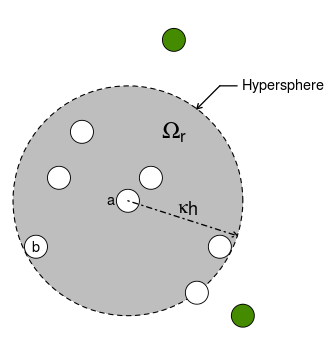
\includegraphics[scale=0.6]{figures/SpInfDiscrete_R.png} 
\caption{{\small{Neighbors List for a Particle ``a''}}}
\label{fig:nearest_neighbors}
\end{figure}

The terms $\mathcal{D}, \mathcal{F}$ and $\mathcal{E}$ are representations of the ``fluxes'' of mass, momentum and energy which contribute to the properties of particle ``a''. Based on the (non-exhaustive) discretizations given in Equations \eqref{eq:Disc_SPH}, PySPH incorporates the following abstractions:

\begin{itemize}
\item \textbf{\textit{Particle Container: }}It is the data structure which represents the arbitrary collections of particles inherent to the SPH method. The material species is represented as a collection of arrays (C++ vectors) describing the required properties. The default particle container comes with representations for the position, velocity, acceleration, pressure, mass, smoothing length and density along with a unique global index(gid), processor id(pid) and a tag\footnote[4]{\url{http://pysph.readthedocs.io/en/latest/reference/particle_array.html}}. Additional properties, if required, can be easily added on the fly. 

\item \textbf{\textit{Nearest Neighbour Queries: }} As mentioned in Section \ref{kappa}, the keeping track of the nearest neighbours of any particle as specified by the hypersphere of influence(Figure \ref{fig:nearest_neighbors}) is computationally the most costly aspect of an SPH simulation. For performing such queries, Nearest Neighbour Particle Search (NNPS) Algorithms are used. By default PySPH implements a Linked List based NNPS; there are however a few more implementations to choose from\footnote[5]{\url{http://pysph.readthedocs.io/en/latest/reference/nnps.html}}.

\item \textbf{\textit{Interaction Physics: }}Based on the specific application area, the physics of the problem defines the nature of the general interaction terms  $\mathcal{D}, \mathcal{F}$ and $\mathcal{E}$ appearing in Equations \ref{eq:Disc_SPH}; there may also be inclusions of viscous stress and artificial viscosity terms for numerical stability of the scheme (more information of details for SPH in specific applications could be found at e.g. \cite{price}, \cite{monaghan_ARFM}, \cite{monaghan_physics},  \cite{volker_springel}). The Interaction Physics abstraction defines with these descriptions in the context of ``solving'' Equations \ref{eq:Disc_SPH} to obtain the accelerations of the particles.

\item \textbf{\textit{Integrator: }}Post completion of the particle interactions, the solution is updated in time using an Integrator\footnote[6]{\url{http://pysph.readthedocs.io/en/latest/reference/integrator.html}} step. These integrators can be include multiple-stages wherein intermediate storage of the properties is inherently available. 

\item \textbf{\textit{Miscellaneous: }}Lastly, data structures, routines and tools to construct solvers, equations, post process the results etc. are required. For post processing, the MayaVi\footnote[7]{\url{http://code.enthought.com/projects/mayavi/}} tool is utilized whereas all other requirements are addressed via routines in the source-code.
\end{itemize} 

\section{Design}

Although superficially it may look like PySPH is written in Python, it is, in reality, a blend of multiple languages. Cython is used to implement the performance critical neighbour queries and pair-wise force computations by creating C/C++ extensions. Further PySPH implements Run Time Code Generation (RTCG) using Python's string processing capabilities to generate OpenCL code on the fly and dynamically compiles it using PyOpenCL\cite{PyOpenCL}. Thus any case setup using PySPH is inherently converted into C/C++ extensions using Cython which ascribes it it's computational edge. Distributed memory computations can be performed via MPI using the Python binding mpi4py \cite{mpi4py} and dynamic load balancing is achieved through the Zoltan data management library \cite{zoltan} via a custom Python wrapper. PySPH can also be seamlessly integrated to use OpenMP for speed-up on systems with multiple cores.

\begin{figure}[htb!]
\centering
\setlength\fboxsep{0pt}
      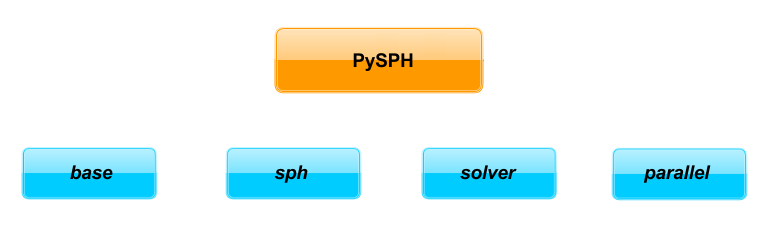
\includegraphics[scale=0.35]{figures/pysph_modules.png} 
\caption{{\small{PySPH subpackages}}}
\label{fig:pysph_modules}
\end{figure}

PySPH comprises of four subpackages as shown in Figure \ref{fig:pysph_modules}. The \textit{base} subpackage contains definitions for the data structures for the particle arrays and nearest neighbour queries on particle sets. The \textit{sph} subpackage contains definitions related to the ``physics'' of the problem. The user's entry point into PySPH is through the  \textit{solver} subpackage wherein provisions are made to facilitate solver construction, choice of the time-stepping scheme and setting of solver parameters. Lastly, the \textit{parallel} subpackage takes care of the domain decomposition, load balancing and computation of remote neighbours using MPI.

Figure \ref{fig:sph_algo} describes the general procedure to setting up a SPH simulation using PySPH.  

\begin{figure}[htb!]
\centering
\setlength\fboxsep{0pt}
      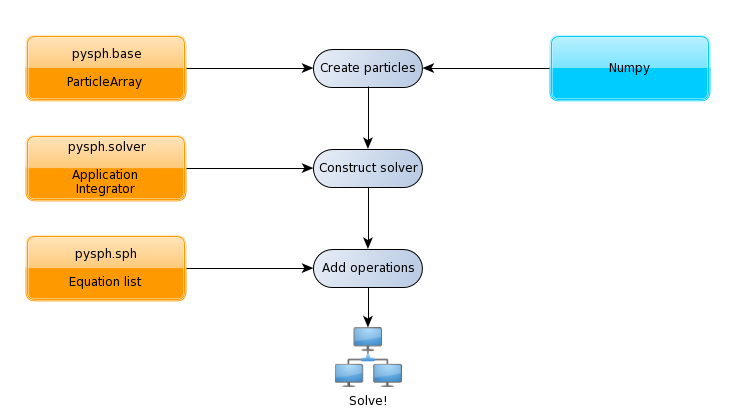
\includegraphics[scale=0.5]{figures/pysph-examples-common-steps.png} 
\caption{{\small{Common Steps}}}
\label{fig:sph_algo}
\end{figure}

To begin with, using Numpy functions in conjunction with the ParticleArray convenience functions Domain Discretization, is performed. Subsequently, the solver is set up wherein details of the Kernel, time step, end time, write frequency etc. are specified along with the choice of integrator scheme to be used. Thereafter, equations which define the interaction physics are constructed and finally solved either serially or in parallel. 

